\documentclass{article}
\usepackage{amsfonts}
\usepackage{amsthm}
\usepackage{amssymb}
\usepackage{amsmath}
\usepackage{graphicx}
\usepackage{subcaption}

\newcommand{\new}[1]{
    \vspace{2mm}
    \noindent
    \textbf{
    \underline{#1}}
}

\def\calO{{\mathcal{O}}}
\def\th{{\theta}}
\def\_{{\hspace{1mm}}}
\def\<{{\langle}}
\def\>{{\rangle}}


\newcounter{problemcnt}
\setcounter{problemcnt}{0}

\newcommand{\Problem}{{
    \vspace{5mm}
    \stepcounter{problemcnt}
    \noindent
    \arabic{problemcnt}. 
}
}

\newcommand{\nProblem}[1]{
    \vspace{5mm}
    \noindent
    \setcounter{problemcnt}{#1}
    \arabic{problemcnt}. 
}


\newcommand{\Proof}{{
    \vspace{2mm}
    \noindent
    \textbf{
    \underline{Proof}}
}
}

\newcommand{\textOr}{
    {
        \hspace{5mm}
        \textrm{or}
        \hspace{5mm}
    }
}

\newcommand{\textAnd}{
    {
        \hspace{5mm}
        \textrm{and}
        \hspace{5mm}
    }
}

\def\Ohm{{\Omega}}

\begin{document}
\begin{center}
\LARGE
PHYS 201 Problemset 10

\Large
Daniel Son
\end{center}

\normalsize

\begin{center}
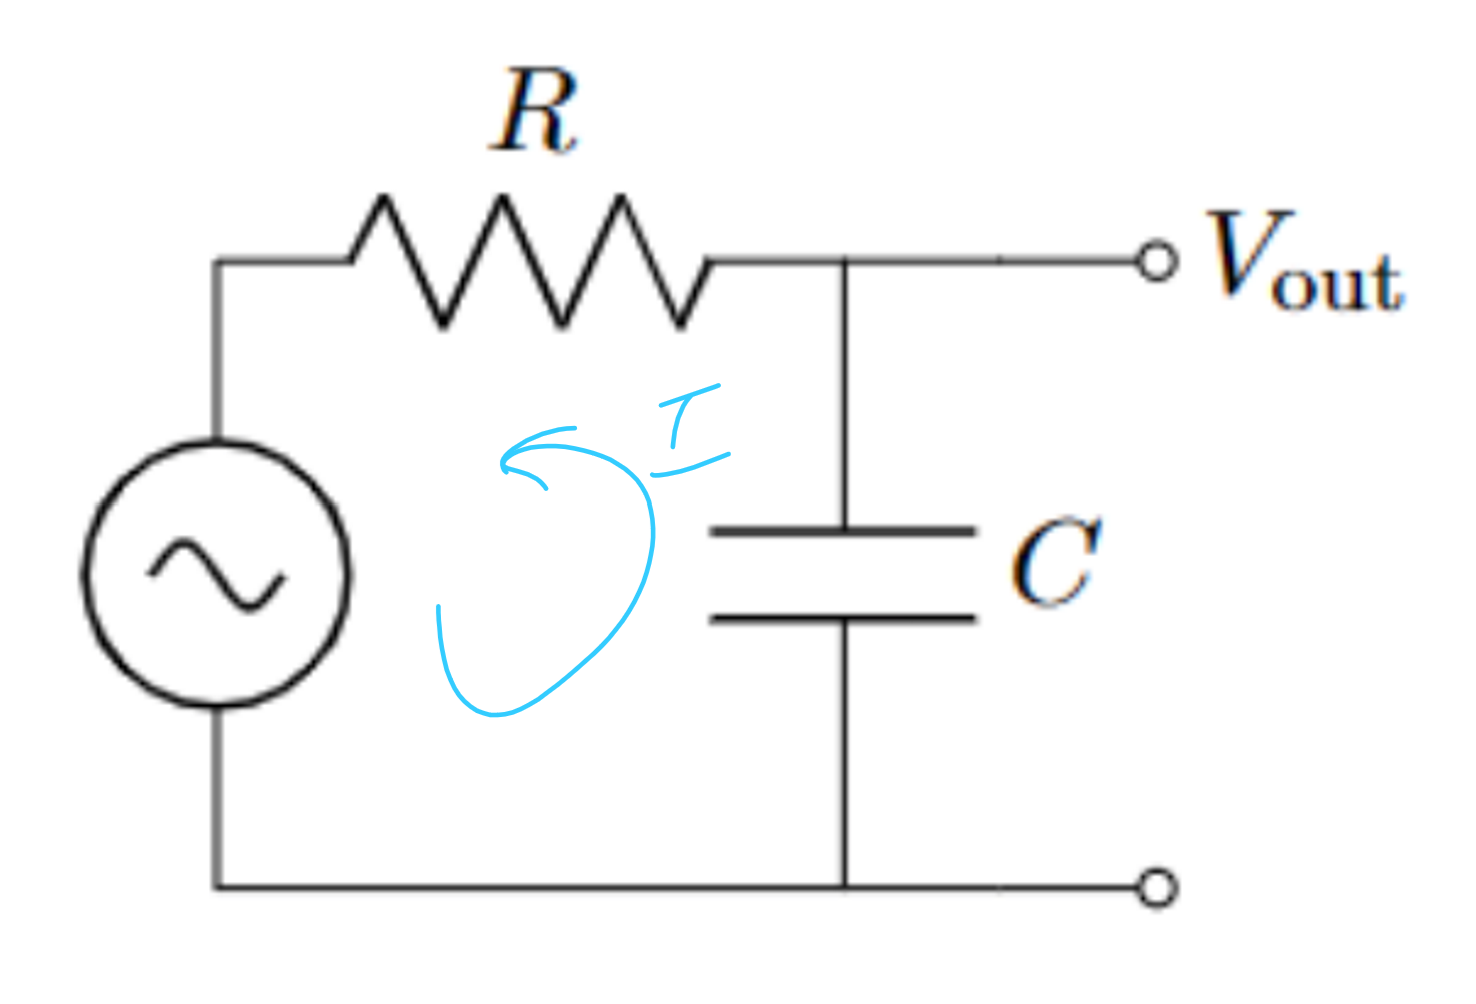
\includegraphics[width = .5\linewidth]{Q1_setup.png}

\textbf{Figrure for Q1}
\end{center}

\new{Q1-a}
Let $V_{in} = V_0 cos(\omega t)$. Use complex impedence to find the 
amplitude of $V_{out}$

\new{Solution}
We know that the loop rule applies to impedences. Write:

\[
    V_0 = \tilde{I}z_R+\tilde{I}z_C
\]

where $z_R, z_C$ denotes the impedence of the capacitor and 
the resistor. By the impedence formula:

\[
    V_0 = \tilde{I}(z_R+z_C)
    \textAnd
    \tilde{I} = \frac{V_0}{R - \frac{i}{\omega C}}
\]

To compute the impedence of $V_out$:

\[
    \tilde{V}_{out} = R\tilde{I} = \frac{RV_0}{R - \frac{i}{\omega C}}
\]

Finally, take the modullus of $\tilde{V}_{out}$ to compute the amplitude.

\[
    \boxed{
    V_{out} = \bigg|
        \frac{RV_0}{R - \frac{i}{\omega C}}
    \bigg|
    = \frac{RV_0}{\sqrt{(R - \frac{i}{\omega C})(R + \frac{i}{\omega C})}}
    = \frac{V_0}{\sqrt{1+\frac{1}{\omega^2 C^2 R^2}}}
    }
\]

\new{Q1-b} Compute the phase shift of $V_{out}$

\new{Solution} 
The phase shift can be easily computed by 
dividing the impedence by amplitude.

\[
    e^{i\theta} = 
    \tilde{V}_{out}/V_{out} 
    = 
R\tilde{I} = \frac{RV_0}{R - \frac{i}{\omega C}}
\bigg/ \frac{V_0}{\sqrt{1+\frac{1}{\omega^2 C^2 R^2}}}
= \frac{\sqrt{1+\frac{1}{\omega^2 C^2 R^2}}}{1 - \frac{i}{\omega CR}}
\]

Thus:
\[
e^{i\theta} 
    = \sqrt{
        \frac{1+\frac{i}{\omega CR}}
    {1-\frac{i}{\omega C R}}
    }
    \textOr
e^{2i\theta} 
    = 
        \frac{1+\frac{i}{\omega CR}}
    {1-\frac{i}{\omega C R}}
\]

With a little bit of geometry, it is possible to deduce:

\[
    2\theta = 2arctan(\frac{1}{\omega CR})
    \textAnd
    \boxed{
    \theta = arctan(\frac{1}{\omega CR})
    }
\]

\qed

\new{Q1-c} Repeat the analysis for a circuit where the 
capacitor is replaced by an inductor. 

\new{Solution}
Rewrite the loop rule as:

\[
    V_0 = \tilde{I}z_{L}+ \tilde{I}z_{R}
    \textAnd 
     V_0 = \tilde{I}(z_L + z_R)
    \textAnd
    \tilde{I} = \frac{V_0}{z_L+z_R}
\]

Applying the impedence formula:

\[
    \tilde{I} = 
    \frac{V_0}
    {i\omega L +R}
    \textAnd
    \tilde{V}_{out} = \frac{V_0R}
    {i\omega L +R}
    = \frac{V_0}{i\omega L/R+1}
\]

Compute the modullus and the argument for the amplitude and 
phase. 

\[
    \boxed{
    V_{out} = |V_{out}| = 
    \frac{V_0}{1+\omega^2L^2/R^2}
    }
\]

With rationalization, $\tilde{V}_{out}$ reduces to:

\[
    \tilde{V}_{out} = \frac{V_0 (1-i\omega L/R)}{(1+i\omega L/R)(1-i\omega L/R)}
    = \frac{V_0(1-i\omega L/R)}{1+\omega^2L^2/R^2}
\]

For the denominator is a real value, it suffices to compute 
the argument of the denominator to compute the argument of the 
impedence. We conclude:
\[
    \boxed{
    \theta = -arctan(\omega L/R)
    }
\]

\new{Q1-d}
A capacitor acts as a short circuit at high-frequency and 
an open circuit at low-frequency. Make an analogous statement 
for inductors.

\new{Statement}
An inductor acts as an open circuit at high-frequency and 
a short circuit at low-frequency. The justification comes 
from observing $V_{out}$ and its dependency on the angular 
frequency, $\omega$. \qed


\newpage
\new{P\&M 8.27}
\textit{RLC Parallel Circuit} A resistor, inductor, capacitor each 
of resistance 1k ohms, 500p farads, 2m henries are connected in 
parallel. The frequency is given as 10k cycles per second. 
Compute the combined impedence of the circuit. Also, compute 
the frequency where the magnitude of impedence is maximal. 

\new{Solution}
For the junction rule holds for impedence, we compute the combined 
impedence by taking the sum of the reciprocals of the impedence 
of each circuit components, and again dividing it from 1. 
In symbols:

\[
    z_{eff} = 
    \frac{1}
    {1/z_c+1/z_l+1/z_r}
\]

where $z_c, z_l, z_r$ denotes the impedence of 
the capacitor, inductor, and resistor respectively. 
Applying the impedence formula:

\[
    z_{eff} = \frac{1}
    {
        \frac{1}{R}
        +
        \frac{1}{i\omega L}
        -
        \frac{\omega C}{i}
    }
    =
    \frac{i \omega LR}
    {i\omega L + R - \omega^2CLR}
\]

The frequency is given as $1kHz$ and $10mHz$, so the angular frequency is:

\[
    \omega_1 = 2\pi \cdot 10^4 Hz
    \textAnd
    \omega_2 = 2\pi \cdot 10^7 Hz
\]

By the problem conditions, we have:
\[
    R = 1000 \Omega
    \textAnd
    C = 5\cdot 10^{-7} F 
    \textAnd
    L = 2\cdot 10^{-3} H
\]

Also, the following unit conversions are useful:
\[
    [C] = F = \Ohm^{-1} \cdot s
    \textAnd
    [L] = H = \Ohm \cdot s
\]

As a sidenote, to derive the two unit conversions, apply dimensional 
analysis on the following formulas:
\[
    Q = CV
    \textAnd
    \mathcal{E} = L\frac{dI}{dt}
\]

With some algebra, with help of python, we conclude:

\[
    \boxed{
    z_{eff} \approxeq 15.7 + 124.2i 
    \textrm{  for 10kHz
    }
    \textAnd
    z_{eff} \approxeq 1.01 -31.8i 
    \textrm{  for 10MHz}
    }
\]

\newpage

\new{Q3}
A mystery device is connected to an AC circuit with 
sinusodial input voltage. The frequency is 100kHz. 
The amplitude of the voltage and current is given as 
$V_0 = 5V, I_0 = 2mA$. The voltage leads the current 
by a phase $\pi/6$. 

\begin{center}
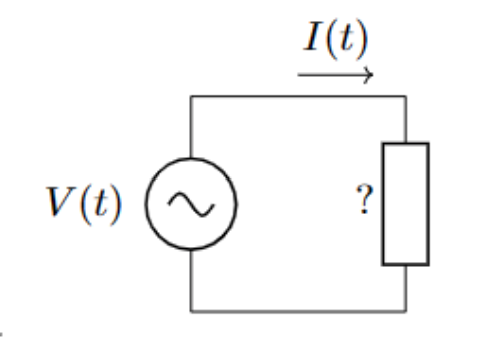
\includegraphics[width = .5\linewidth]{Q3_setup.png}

\textbf{
Circuit image for Q3
}
\end{center}

i) Compute the impedence of the mystery device

\new{Solution}

Write:

\[
    \tilde{V} = 5V
    \textAnd
    \tilde{I} = 2mA e^{-i\pi/6}
\]

Thus:

\[
    z = \tilde{V}/\tilde{I} = 2.5\cdot10^3 e^{i\pi/6} \Ohm
\]

Or, in cartesian form:
\[
    \boxed{
        z = (2170+1250i)\Ohm
    }
\]

ii) What is a potential candidate for this mystery device?

\new{Solution}
An equivalent of the device can be constructed 
by connecting a resistor with a resistor. Denote the 
resistance and the inductor as $R, L$. The combined 
impedence of connecting the two components in series is:

\[
    z_{cmb} = R + i\omega L
\]

We deduce:
\[
    R = 2170\Ohm 
    \textAnd 
    \omega L  = 2\pi f L = 1250 \Ohm
\]

Ergo:
\[
    \boxed{
        R = 2170\Ohm 
        \textAnd
        L = 2mH
    }
\]

iii) Assume that the mystery device is indeed composed of 
the elements that were guessed in the previous problem. 
How will the amplitude of current change as the frequency 
is increased? Moreover, how will the change of frequency 
affect the phase difference between the voltage and current?

\new{Solution}
As frequency increases, $\omega$ increases. This results 
in an increase of both the argument and the magnitude of 
the impedence. Recall:

\[
    z = \tilde{V}/\tilde{I}
    \textOr 
    \tilde{I} = \tilde{V}/z
\]

Hence, larger magnitude of impedence leads to decrease of 
the amplitude of the current. Also, the larger the argument 
of the impedence, the larger the phase difference between 
voltage and current. 
\qed

\new{Prelude to Q4}
When talking about power in AC circuits, it is convinient 
to use root mean squared values for voltage and current. Note that 
RMS is NOT EQUAL to the simple mean. 

Two following equations come in handy:
\[
    \bar{P} = V_{rms}^2/R
    \textAnd
    \bar{P} = V_{rms}I_{rms}cos(\phi)
\]

As part of being physicists, we leave it as an exercise to 
the mathematicians to justify this equation. 

To compute the rms value of a sinusodial function, remember:

\[
    A_{rms} = A_0/\sqrt{2}
\]

where $A_0$ denotes the amplitude of the quantity. 

\new{Q4}
An incandecent bulb consumes $60W$ of power if connected to 
a standard $120V, 60Hz$ AC circuit. We wish to connect this 
bulb to a circuit with $240V, 60Hz$ voltage and frequency. 
By connecting an inductor in series with the bulb, it is possible 
to make the bulb consume the same amount of power in average. 
What must be the inductance of the inductor?

\new{Solution}
The bulb has an internal resistance. This can be easily computed 
by the power formula. Write:

\[
    P = V_{rms}^2/R 
    \textAnd 
    R = V_{rms}^2/P = (120V)^2/60W = 240\Ohm
\]

If the bulb is connected in series with an inductor, the 
magnitude of the combined impedence increases. Let 
$L$ denote the inductance of the inductor. Write:

\[
    z_{eff} = i\omega L + R
\]
\[
    \tilde{I} = V/z_{eff} \textAnd \tilde{V}_b = \tilde{I}R = \frac{VR}{z_{eff}}
\]
Thus
\[
    V_b = \frac{VR}
    {|i\omega L + R|}
    = 
    \frac{VR}
    {\sqrt{R^2+\omega^2L^2}}
    = 
    \frac{V}
    {\sqrt{1+\omega^2 (L/R)^2}}
\]

where $V_b$ denotes the voltage through the bulb. 

If $V_b = 120V$, then the bulb consumes the same power as 
connected to the standard circuit. $V = 240V$ so we wish 
to fix the denominator as 2. Then:

\[
\sqrt{1+\omega^2 (L/R)^2} = 2
\textOr 
1+\omega^2(L/R)^2 = 4
\]

So:

\[
    L^2 = 3R^2/\omega^2 
    \textAnd 
    L = \sqrt{3}R/\omega
\]

Ergo:
\[
    \boxed{
        L \approxeq 1.1H
    }
\]  



\end{document}